\def\year{2022}\relax
%File: formatting-instructions-latex-2022.tex
%release 2022.1
\documentclass[letterpaper]{article} % DO NOT CHANGE THIS
\usepackage{aaai22}  % DO NOT CHANGE THIS
\usepackage{times}  % DO NOT CHANGE THIS
\usepackage{helvet}  % DO NOT CHANGE THIS
\usepackage{courier}  % DO NOT CHANGE THIS
\usepackage[hyphens]{url}  % DO NOT CHANGE THIS
\usepackage{graphicx} % DO NOT CHANGE THIS
\urlstyle{rm} % DO NOT CHANGE THIS
\def\UrlFont{\rm}  % DO NOT CHANGE THIS
\usepackage{natbib}  % DO NOT CHANGE THIS AND DO NOT ADD ANY OPTIONS TO IT
\usepackage{caption} % DO NOT CHANGE THIS AND DO NOT ADD ANY OPTIONS TO IT
\DeclareCaptionStyle{ruled}{labelfont=normalfont,labelsep=colon,strut=off} % DO NOT CHANGE THIS
\frenchspacing  % DO NOT CHANGE THIS
\setlength{\pdfpagewidth}{8.5in}  % DO NOT CHANGE THIS
\setlength{\pdfpageheight}{11in}  % DO NOT CHANGE THIS
%
% These are recommended to typeset algorithms but not required. See the subsubsection on algorithms. Remove them if you don't have algorithms in your paper.
\usepackage{algorithm}
\usepackage{algorithmic}

%
% These are are recommended to typeset listings but not required. See the subsubsection on listing. Remove this block if you don't have listings in your paper.
\usepackage{newfloat}
\usepackage{listings}
\lstset{%
	basicstyle={\footnotesize\ttfamily},% footnotesize acceptable for monospace
	numbers=left,numberstyle=\footnotesize,xleftmargin=2em,% show line numbers, remove this entire line if you don't want the numbers.
	aboveskip=0pt,belowskip=0pt,%
	showstringspaces=false,tabsize=2,breaklines=true}
\floatstyle{ruled}
\newfloat{listing}{tb}{lst}{}
\floatname{listing}{Listing}
%
%\nocopyright
%
% PDF Info Is REQUIRED.
% For /Title, write your title in Mixed Case.
% Don't use accents or commands. Retain the parentheses.
% For /Author, add all authors within the parentheses,
% separated by commas. No accents, special characters
% or commands are allowed.
% Keep the /TemplateVersion tag as is
\pdfinfo{
/Title (Model-Based Adaptation to Novelty in Open-World AI)
/Author (Wiktor Piotrowski, Roni Stern, Matthew Klenk, Alexandre Perez, Johan de Kleer, Jacob le, Shiwali Mohan)
/TemplateVersion (2022.1)
}

% DISALLOWED PACKAGES
% \usepackage{authblk} -- This package is specifically forbidden
% \usepackage{balance} -- This package is specifically forbidden
% \usepackage{color (if used in text)
% \usepackage{CJK} -- This package is specifically forbidden
% \usepackage{float} -- This package is specifically forbidden
% \usepackage{flushend} -- This package is specifically forbidden
% \usepackage{fontenc} -- This package is specifically forbidden
% \usepackage{fullpage} -- This package is specifically forbidden
% \usepackage{geometry} -- This package is specifically forbidden
% \usepackage{grffile} -- This package is specifically forbidden
% \usepackage{hyperref} -- This package is specifically forbidden
% \usepackage{navigator} -- This package is specifically forbidden
% (or any other package that embeds links such as navigator or hyperref)
% \indentfirst} -- This package is specifically forbidden
% \layout} -- This package is specifically forbidden
% \multicol} -- This package is specifically forbidden
% \nameref} -- This package is specifically forbidden
% \usepackage{savetrees} -- This package is specifically forbidden
% \usepackage{setspace} -- This package is specifically forbidden
% \usepackage{stfloats} -- This package is specifically forbidden
% \usepackage{tabu} -- This package is specifically forbidden
% \usepackage{titlesec} -- This package is specifically forbidden
% \usepackage{tocbibind} -- This package is specifically forbidden
% \usepackage{ulem} -- This package is specifically forbidden
% \usepackage{wrapfig} -- This package is specifically forbidden
% DISALLOWED COMMANDS
% \nocopyright -- Your paper will not be published if you use this command
% \addtolength -- This command may not be used
% \balance -- This command may not be used
% \baselinestretch -- Your paper will not be published if you use this command
% \clearpage -- No page breaks of any kind may be used for the final version of your paper
% \columnsep -- This command may not be used
% \newpage -- No page breaks of any kind may be used for the final version of your paper
% \pagebreak -- No page breaks of any kind may be used for the final version of your paperr
% \pagestyle -- This command may not be used
% \tiny -- This is not an acceptable font size.
% \vspace{- -- No negative value may be used in proximity of a caption, figure, table, section, subsection, subsubsection, or reference
% \vskip{- -- No negative value may be used to alter spacing above or below a caption, figure, table, section, subsection, subsubsection, or reference







% Use the postscript times font!
% \usepackage{times}
% \usepackage{soul}
% \usepackage{url}
% \usepackage[hidelinks]{hyperref}
% \usepackage[utf8]{inputenc}
% \usepackage[small]{caption}
% \usepackage{graphicx}
% \usepackage{amsmath}
% \usepackage{amsthm}
% \usepackage{booktabs}
% \usepackage{algorithm}
% \usepackage{algorithmic}
% \urlstyle{same}
\linespread{0.99}

\usepackage{amsmath,amssymb,amsfonts} % Added for HYDRA
\newcommand{\tuple}[1]{\ensuremath{\left \langle #1 \right \rangle }} % Added for HYDRA
\newcommand{\reals}{\ensuremath{\mathbb{R}}} % Added for HYDRA
\usepackage[obeyFinal,final]{todonotes} % Added for HYDRA
\usepackage{xspace} % Added for HYDRA
\newcommand{\sbirds}{Science Birds\xspace} % Added for HYDRA % TODO Replace with acronym
\newcommand{\hydra}{\textsc{Hydra}\xspace} % Added for HYDRA % TODO Replace with acronym
\newtheorem{definition}{Definition} % Added for HYDRA




\setcounter{secnumdepth}{0} %May be changed to 1 or 2 if section numbers are desired.

% The file aaai22.sty is the style file for AAAI Press
% proceedings, working notes, and technical reports.
%

% Title

% Your title must be in mixed case, not sentence case.
% That means all verbs (including short verbs like be, is, using,and go),
% nouns, adverbs, adjectives should be capitalized, including both words in hyphenated terms, while
% articles, conjunctions, and prepositions are lower case unless they
% directly follow a colon or long dash
\title{Model-Based Adaptation to Novelty in Open-World AI}
\author{
    %Authors
    % All authors must be in the same font size and format.
    Roni Stern,\textsuperscript{\rm 1,2}\equalcontrib
    Wiktor Piotrowski,\textsuperscript{\rm 1}\equalcontrib
    Matthew Klenk,\textsuperscript{\rm 3}\equalcontrib
    Johan de Kleer,\textsuperscript{\rm 1}
    Alexandre Perez,\textsuperscript{\rm 1}
    Jacob Le,\textsuperscript{\rm 1} 
    Shiwali Mohan\textsuperscript{\rm 1} \equalcontrib
}
\affiliations{
    %Afiliations
    \textsuperscript{\rm 1} Palo Alto Research Center, CA, USA\\
    \textsuperscript{\rm 2} Ben-Gurion University of the Negev, Beer-Sheva, Israel\\
    \textsuperscript{\rm 3} Toyota Research Institute, CA, USA\\
    e-mail: roni.stern@gmail.com;\{wiktorpi,smohan,dekleer,jale\}@parc.com;matt.klenk@tri.global;alexandrecperez@gmail.com\\
}


%Example, Single Author, ->> remove \iffalse,\fi and place them surrounding AAAI title to use it
\iffalse
\title{My Publication Title --- Single Author}
\author {
    Author Name
}
\affiliations{
    Affiliation\\
    Affiliation Line 2\\
    name@example.com
}
\fi

\iffalse
%Example, Multiple Authors, ->> remove \iffalse,\fi and place them surrounding AAAI title to use it
\title{My Publication Title --- Multiple Authors}
\author {
    % Authors
    First Author Name,\textsuperscript{\rm 1}
    Second Author Name, \textsuperscript{\rm 2}
    Third Author Name \textsuperscript{\rm 1}
}
\affiliations {
    % Affiliations
    \textsuperscript{\rm 1} Affiliation 1\\
    \textsuperscript{\rm 2} Affiliation 2\\
    firstAuthor@affiliation1.com, secondAuthor@affilation2.com, thirdAuthor@affiliation1.com
}
\fi


% REMOVE THIS: bibentry
% This is only needed to show inline citations in the guidelines document. You should not need it and can safely delete it.
\usepackage{bibentry}
% END REMOVE bibentry

\begin{document}

\maketitle

\begin{abstract}
Most model-based agents are ill-equipped to handle novel situations in which their model of the environment no longer sufficiently represents the world. 
We introduce \hydra, an architecture for a model-based agent operating in open-world, mixed continuous-discrete environments that detects and effectively adapts to novelties encountered during performance. 
\hydra does so by using a compositional model of the environment and employing a range of AI techniques including domain-independent automated planning, anomaly detection, model-based diagnosis, and heuristic search. We also present a design for a \hydra agent that uses PDDL+, a rich domain-independent planning domain description language, to define its compositional model. 
An empirical evaluation on the well-known balancing cartpole problem, a standard Reinforcement Learning (RL) benchmark, demonstrates that our PDDL+-based \hydra agent is able to quickly and effectively detect and adapt to some classes of novelties, outperforming an off-the-shelf deep q-network (DQN) agent. 
\end{abstract}


\section{Introduction}

% MAIN BODY


% Motivation: novelty is key to intelligence

%While current AI systems perform with superhuman capability in many game domains, each of these domains is a closed world, and minor perturbations of the game can lead to significant drops in performance. Witty et al.~\shortcite{witty2018measuring} demonstrated that even changes which made the game easier could cause catastrophic results for superhuman performing deep Q-learning agents. On the other hand, 

One hallmark of human cognition is our ability to function in an open world. 
People navigate to previously unseen places, perform new tasks, and integrate new technology into their lives. In games, human flexibility supports inventing new strategies along with adapting to changing rules. \todo{If there's a nice humanities-type of reference here that'd be great.}
% (e.g., consider chess players who play bughouse\footnote{\url{https://en.wikipedia.org/wiki/Bughouse_chess}}).\todo{I'm considering removing the bughouse example. Comments?}
In contrast, current AI systems perform with superhuman capability in many closed-world game domains, but minor perturbations of the game can lead to significant drops in performance. 
For example, Witty et al.~\shortcite{witty2018measuring} demonstrated that even changes which made the game easier could cause catastrophic results for superhuman-performing deep Q-learning agents. 
This mismatch between human cognitive abilities and machine capabilities indicates that effectively responding to novelty is a major problem in current AI systems~\cite{senator2019sailon}. 


In this work, we explore the novelty response problem in the context of an autonomous agent acting in the world. 
The agent performs actions, collects observations, and accumulates rewards which it aims to maximize. 
At some stage, a novelty is introduced, that is, the dynamics of the environment changes. 
To continue to function effectively, the agent must adapt its behavior. 
A naive approach for this novelty response problem is to re-train the agent on the modified environment using an off-the-shelf RL algorithm. 
Yet, such re-training may require numerous interactions with the environment and ignores knowledge about aspects of the environment that has not changed. 
\todo[inline,color=green]{TODO: Add a bit of text on lifelong RL and how it relates. Something that will go like this: ``Black-box lifelong RL are designed for ... but it is difficult to incorporate background knowledge of the environment to these methods [[and maybe something more about them]]''}


The first contribution of this work is \hydra, a model-based architecture of an autonomous agent that plans and acts effectively in a changing environment. 
A key element in the \hydra architecture is the use of a \emph{compositional model} of the environment, i.e., a model whose components represent meaningful aspects of the environment, as opposed to a black-box prediction model such as a deep neural network. 
This compositional model is used to plan which actions to perform, but also to monitor their execution and detect novelties by comparing the outcomes of executed actions with the model's expectation. 
When novelty is detected, the \hydra agent responds by employing a model-based diagnosis engine to identify the components of its compositional model that need to be adapted to be consistent with detected novelties. 
The main benefit of using a compositional model is that planning is more robust to changes and adapting to novelty does not require re-training the agent from scratch. 

% such that it is consistent with collected observations. 

% It then adapts to novelty quickly by modifying the surrogate model accordingly. 

% byusing and automated planner, 
% Central in the \hydra to the design of a \hydra agent is a \emph{compositional model} of the environment, i.e., a model whose components represent meaningful aspects of the environment, as oppose to a black-box prediction model such as a deep neural network. 
% This compositional model is used byusing and automated planner, 
% and monitor their execution. 


% wh

% to detect novelties by comparing the outcomes of executed actions with the model's expectation. 

% monitor their execution. 

% , follow their 
% This surrogate model is used not only for planning which actions to perform, but also to detect novelties by comparing the outcomes of executed actions with the model's expectation. When novelty is detected, the \hydra agent responds by employing a model-based diagnosis engine to identify the components of its surrogate model that need to be modified such that it is consistent with collected observations. It then adapts to novelty quickly by modifying the surrogate model accordingly. 



% including how different objects in the environment are affected by agent's actions. 
% This model is used 

% \emph{compositional model} of the environment and selects actions by applying providing this model to an automated planning algorithm. 

% n environment and can effectively detect and adapt to novel changes in the environment. A \hydra agent follows a model-based approach, maintaining a surrogate model of the environment and selects actions by applying providing this model to an automated planning. This surrogate model is composable, as oppose to a black-box deep neural network prediction model, i.e., the components of the model represent meaningful aspects of the environment, including how different objects in the environment are affected by agent's actions. This surrogate model is used not only for planning which actions to perform, but also to detect novelties by comparing the outcomes of executed actions with the model's expectation. When novelty is detected, the \hydra agent responds by employing a model-based diagnosis engine to identify the components of its surrogate model that need to be modified such that it is consistent with collected observations. It then adapts to novelty quickly by modifying the surrogate model accordingly. 

%The first contribution of this work is \hydra, an architecture for an autonomous agent that effectively detects and adapts to novel changes in the environment. A \hydra agent follows a model-based approach, maintaining a surrogate model of the environment and selects actions by applying providing this model to an automated planning. This surrogate model is composable, as oppose to a black-box deep neural network prediction model, i.e., the components of the model represent meaningful aspects of the environment, including how different objects in the environment are affected by agent's actions. This surrogate model is used not only for planning which actions to perform, but also to detect novelties by comparing the outcomes of executed actions with the model's expectation. When novelty is detected, the \hydra agent responds by employing a model-based diagnosis engine to identify the components of its surrogate model that need to be modified such that it is consistent with collected observations. It then adapts to novelty quickly by modifying the surrogate model accordingly. 

%not a black-box, and \hydra is aware of  prediction model. compositional, that is 
% to novelty detection and response. 
%\hydra separates the response to novelty into two subproblems: \textbf{novelty detection} and \textbf{novelty response}. he design of \hydra is focused on addressing two key subproblems: \textbf{novelty detection} and \textbf{novelty response}. Novelty detection is the problem of identifying from the collected observations whether something meaningfully novel has occurred~\cite{pimentel2014review}. Novelty response is the problem of adapting the behavior of the agent when novelty is introduced such that it continues to function effectively. While each of these problems, individually, have been addressed in the literature to some extent, \hydra solves them in a synergetic manner and in the context of acting in a dynamically-changing mixed continuous-discrete world. 
%In addition, performing these tasks in the mixed a continuous-discrete environment in which \hydra operates is very challenging. \todo[inline,color=green]{[[Roni: maybe add a bit more here in terms of related works]]}
% 
% Concrete: we develop an agent that works in a mixed continuosu-discrete environment, can perform actions and get observations. 
% As a step towards this goal, we developed the \textbf{Hypothesis-Guided Model Revision over Multiple Aligned Representations} (\hydra) agent. 
% First contribution: design
%The first contribution of this work is \hydra, a model-based agent designed to effectively detect and respond to novelties using very few interactions. 
%The \hydra model is a composable surrogate model} of the environment that enables making predictions over the outcomes of the agent's actions. 
%that approximates the environment's dynamics, and
%tennents architecture \hydra of a model-based agent 

%\hydra design, which follows a model-based approach to novelty detection and response. It maintains a surrogate model of the world dynamics and selects actions by applying providing this model to an automated planning. Then, it tracks the execution of these plans, and detects novelties in the world when the outcomes of planned actions differ from the model's expectation. When novelty is detected, \hydra responds by employing a model-based diagnosis engine to identify the aspects of the surrogate world model that needs to be modified such that it is consistent with collected observations. Future actions are adapted to the novelty as they are planned according to the modified surrogate world. 



%Indeed, adapting to novelty is a major challenge for current AI systems. 
%Our research goal is to impart machines with human-like learning capabilities to make them robust to novelty. 



% The problem of adapting to novelty encompasses two sub-problems: \textbf{novelty detection} and \textbf{novelty response}.
% Novelty detection is the problem of detecting \emph{when} something meaningfully novel has occurred~\cite{pimentel2014review}. 
% Novelty response is the problem of adapting the behavior of the agent when novelty is introduced such that it continues to function effectively. While each of these problems, individually, have been addressed in the literature to some extent, \hydra solves them in a synergetic manner and in the context of acting in a dynamically-changing mixed continuous-discrete world. 
% %In addition, performing these tasks in the mixed a continuous-discrete environment in which \hydra operates is very challenging. 
% \todo[inline,color=green]{[[Roni: maybe add a bit more here in terms of related works]]}
% % 





% The topic of how to detect and react to novelties has been gaining significant attention in the AI literature. 
% The novelty problems we address in this work has been described by Senator~\cite{senator2019sailon} 
% and analyzed by Boult et al.~\cite{boult2021towards}
% and Langely~\cite{langley2020open}. 
% Boult et al.~\cite{boult2021towards,langley2020open} did not propose an agent design for this setting, but rather suggested a framework for characterizing different types of novelties. 


% Langely also identified four elements an agent architecture needs to properly address novelty detection and response --- ``performance, monitoring, diagnosis, and repair.'' 
% \hydra implements these elements. 
% It uses its meta model to generate plans, act (\emph{performance}), and detect novelties (\emph{monitor}). 
% Then, it uses heuristic search to identify elements of the meta model that are incorrect (\emph{diagnosis}) and modifies the meta model accordingly (\emph{repair}). 

% We are not the first to design a novelty-robust agent and novelty detection and response algorithms. DiscoverHistory~\cite{molineaux2012discoverhistory} is an algorithm for inferring the possible values of unobservable state variables from observations. While our current experiments are similar in nature, HYDRA is designed to be more general, including novelties such as adding new variables, process, and object types. MIDCA~\cite{paisner2014goal} is a cognitive architecture for designing novelty-robust agents, where novelty is limited to which goal to pursue next. 










% Second contribution: implementation in PDDL+
Our second contribution is a complete implementation of a \hydra agent that uses PDDL+~\cite{fox2006modelling} to represent its compositional environment model. % \hydra's beliefs about the environment dynamics. 
PDDL+ is a feature-rich domain-independent planning modeling language that has been used to model a range of complex planning problems, including Chemical Batch Plant~\cite{della2010pddl+}, Atmospheric Reentry~\cite{piotrowski2018heuristics}, Urban traffic Control~\cite{vallati2016efficient}, and Planetary Lander~\cite{della2010resource}. 
Using PDDL+ allows such a \hydra agent to be used in a broad range of domains, including domains that require discrete and continuous state variables as well as exogenous events and continuous processes. 
We describe our PDDL+-based \hydra agent in detail, and highlight the challenges in doing so. 
% Third contribution: experiments. 
The third contribution of this paper is an empirical evaluation of a PDDL+-based \hydra agent on a standard Reinforcement Learning (RL) benchmark - OpenAI Gym's balancing Cartpole domain~\cite{barto1983neuronlike,brockman2016openai}. Our results show that \hydra is \emph{resilient} to novelties; i.e, the degradation in its performance is not as severe as the standard deep Q-network (DQN) RL agent. Second, we show that \hydra adapts \emph{quickly}, requiring less than $20$ episodes to return to top performance after novelty has been introduced, much faster than the DQN RL agent. Finally, adaptations in \textsc{hydra} are \emph{interpretable}. They are represented in terms of changes to the elements of its domain model enabling inspection of proposed changes.
\todo{Above paragraphs modified, please re-read}

% of this is a demonstration of 

% how a PDDL+-based \hydra agent dcan adapt rapidly adapts to novelties

% our PDDL+ \hydra implementation on a standard standard Reinforcement Learning (RL) benchmark, namely, OpenAI Gym's balancing Cartpole domain~\cite{barto1983neuronlike,brockman2016openai}. 
% The results show that \hydra can adapt to novelty much faster than a standard Reinforcement Learning (RL) technique, requiring only five  episodes to return to top performance after novelty has been introduced. 
% %Finally, we describe key challenges that arise when using \hydra in other domains and outline directions to meet these challenges. 







% on the well-known OpenAI Gym's balancing Cartpole domain~\cite{brockman2016openai}. 


% \hydra is a model-based agent: it uses a surrogate model of the world to plan its actions and to identify when the outcomes of executed actions differ from the model's expectation. It employs model-based diagnosis to diagnose the root cause of such discrepancies, and adapts to novelty by adapting that surrogate model such that it is consistent with collected observations. 

% Central to our design is the \emph{meta model}, which maps between To maintain a domain-independent design




% To maintain a domain-independent design, we based our implementation of \hydra on  PDDL+~\cite{fox2006modelling}, a feature-rich domain-independent planning modeling language, to represent \hydra's beliefs about the environment dynamics. 
% PDDL+ is an extension of the well-known Planning Domain Definition Language (PDDL)~\cite{mcdermott1998pddl} that allows defining discrete and continuous state variables as well as exogenous events and continuous processes. 
% It has been used to model a range of complex planning problems, including Chemical Batch Plant~\cite{della2010pddl+}, Atmospheric Reentry~\cite{piotrowski2018heuristics}, Urban traffic Control~\cite{vallati2016efficient}, and Planetary Lander~\cite{della2010resource}.
% % \todo[inline,color=green]{[[Roni: todo - fill with references of applications]]}



% A central component in \hydra is a 

% selects which actions to perform by
% invoking a domain-independent PDDL+ planner over 
% the agent's PDDL+ model of the environment and the task at hand. 
% Novelty detection is performed by comparing the expected outcome of the actions it performed %according to \hydra's PDDL+ model and 
% with the observed outcome.  
% Novelty response is performed by automatically diagnosing and then repairing \hydra's PDDL+ model so that it is consistent with the observations. 




% % Key: PDDL+ model of the world 
% Central to our approach for both novelty detection and adaptation is the use of PDDL+~\cite{fox2006modelling}, a feature-rich domain-independent planning modeling language, to represent \hydra's beliefs about the environment dynamics. 
% PDDL+ is an extension of the well-known Planning Domain Definition Language (PDDL)~\cite{mcdermott1998pddl} that allows defining discrete and continuous state variables as well as exogenous events and continuous processes. 
% It has been used to model a range of complex planning problems, including Chemical Batch Plant~\cite{della2010pddl+}, Atmospheric Reentry~\cite{piotrowski2018heuristics}, Urban traffic Control~\cite{vallati2016efficient}, and Planetary Lander~\cite{della2010resource}.
% % \todo[inline,color=green]{[[Roni: todo - fill with references of applications]]}
% \hydra selects which actions to perform by
% invoking a domain-independent PDDL+ planner over 
% the agent's PDDL+ model of the environment and the task at hand. 
% Novelty detection is performed by comparing the expected outcome of the actions it performed %according to \hydra's PDDL+ model and 
% with the observed outcome.  
% Novelty response is performed by automatically diagnosing and then repairing \hydra's PDDL+ model so that it is consistent with the observations. 



% % Experiments
% We have implemented \hydra on two domains: OpenAI Gym's balancing Cartpole domain~\cite{brockman2016openai}, and Science Birds, a version of the popular Angry Birds game developed for research purposes~\cite{renz2019ai}. 
% In this work, we describe our implementation for Cartpole and report on a small-scale set of experiments in the Cartpole domain. The results show that \hydra can adapt to novelty much faster than standard Reinforcement Learning (RL) techniques, requiring only \todo[inline,color=green]{[[TODO: HOW MANY]]} interactions with the world to return to top performance after novelty has been introduced. Then, we describe key challenges that arise when using \hydra for ScienceBirds, and outline directions to meet these challenges. 


\section{Problem Definition}

% The general setting of the world
\hydra is designed to interact with the environment in a standard RL setup. 
That is, the agent plays a sequence of \textbf{episodes}, 
every episode consists of a sequence of \textbf{steps},
and every step consists of observing a state, 
performing an action, 
observing the resulting state, 
and receiving reward. 
The reward of an episode is the sum of rewards in its constituent steps.
We assume that the \emph{environment} is a transition system $E=\tuple{S, A, S_I, S_T, R}$
where $S$ is the possibly infinite set of states;
$A$ is the set of possible actions; 
$S_I\subseteq S$ is a set of possible initial states, 
$S_T\subseteq S$ is set of terminal states, 
and $R$ is a reward function $R: S\rightarrow \reals$, where $R(s)$ returns the reward of reaching state $s$.\footnote{Other reward function formulations are also common, e.g., where the reward function includes both state and action ($R(s,a)$).}
An agent plays an episode in the environment $E$ 
means that the agent selects and performs an action in the environment starting 
from a randomly selected initial state $s_I\in S_I$ and ending when reaching a terminal state $s_T\in S_T$. 
The result of an agent playing an episode is a \emph{trajectory}, which comprises a sequence of tuples of the form $\tuple{s, a, s',r}$, representing that the agent performed action $a$ at state $s$, reached the state $s'$ and collected a reward $r$. 




% Defining novelty
Following the \emph{Theory of Environmental Change}~\cite{langley2020open}, 
we view \emph{novelty} as a transformation of the underlying environment $E$ that occurs at some point in time.
Formally, we consider novelty here as a function $\varphi$ that can be applied to an environment $E$ and outputs an environment $\varphi(E)$ 
that is different from $E$ in some way.\footnote{Boult et al.~\cite{boult2021towards} referred to this type of novelty as a \emph{world novelty}.}
Introducing a novelty $\varphi$ in an environment $E$ means that the underlying environment $E$ changes to $\varphi(E)$. 
In an open world, sequences of novelties can, in general, be introduced at multiple points in time. 
However, in this work we impose constraints and assume that 
(1) novelty is not introduced during an episode, only between episodes;
(2) at most one novelty will be introduced;
(3) once a novelty is introduced all subsequent episodes are played in the modified environment. 
We refer to this setup as the \emph{single persistent novelty setup}. 

\begin{definition}[The Novelty Response Problem]
A novelty response problem is defined by a tuple $\Pi=\tuple{E, \varphi, t_N}$ 
where $E$ is a transition system, $\varphi$ is a novelty function, 
and $t_N$ is a non-negative integer specifying the episode in which novelty $\varphi$ is introduced. 
In this setup, an agent plays $t_N$ episodes from environment $E$ 
and all subsequent episodes in environment $\varphi(E)$. 
\end{definition}

% Objective
The objective of an agent faced with this novelty response problem is to maximize its cumulative reward over time. 
A key challenge for an agent of this setup is that the agent does know the values of neither $t_N$ nor $\varphi$. 
That is, the agent does not known \emph{when} novelty will be introduced and \emph{how} it will change the environment. Next, we describe \hydra, our proposed architecture for a model-based agent faced with a novelty response problem. 

%We focus on two challenges that arise in this setup when an agent plays multiple episodes: \emph{novelty detection} and \emph{novelty response}.  The former challenge refers to identifying which episodes are played in $\varphi(E)$  and the latter challenge refers to maximizing the rewards collected over time. 
% Our objective is to play the game, \emph{detect} the novelty when it occurs, and \emph{respond} to it. 
% We define these objectives formally as follows. 
% Let $e_1,\ldots$ be a sequence of episodes, and let $e_n$ be the first episode in which novelty has been introduced. %
%Note that to directly address the novelty detection challenge, the game playing agent outputs its belief about whether or not novelty has been introduced after playing every episode. 


% An example of novelty is the introduction of a new bird type with different dynamics and actions that would be available in future levels. 





% \begin{figure}[bth]
% \centering
%         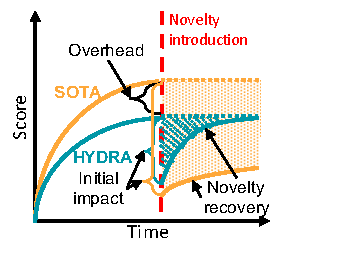
\includegraphics[width=0.75\columnwidth]{figures/Metrics.pdf}
%         \caption{An illustration of the desired novelty response behavior. The $x$-axis is time --- number of episodes played --- and the $y$-axis is the reward collected in every played episode.}
%         \label{fig:hydra-metrics}
% \end{figure}
%For novelty detection, performance can be measured using standard anomaly detection metrics (false positives, false negatives, etc.). 



% \begin{figure*}[bth]
% \center{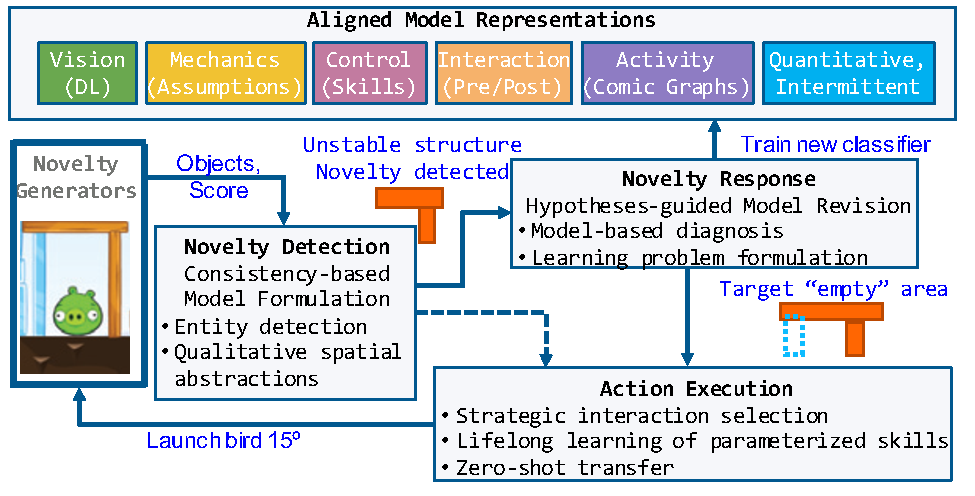
\includegraphics[scale=0.7]{figures/HYDRA.pdf}}
% \vspace{-0.3cm}
%         \caption{\label{fig:hydra} HYDRA draws on multiple model representations to plan actions, observe their effects, and focus learning.}
% \end{figure*}
% Figure~\ref{fig:hydra-metrics} illustrates the desired behavior of our agent, in terms of novelty response. 
% The $x$-axis is number of episodes played (``Time'') 
% and the $y$-axis is the reward collected in every played episode (``Score''). 
% The vertical dashed red line marks when novelty has been introduced. 
% The SOTA line illustrate how a standard state of the art learning agents is expected to behave before and after novelty has been introduced. 
% We expected the SOTA's performance to significantly decrease when some novelties are introduced, and that it would require significant re-training for the SOTA agent to return to high performance. This degraded performance between the time novelty has been introduced and the agent fully adapts to it is referred to as the \textbf{novelty recovery} penalty. Hydra is designed to minimize this penalty, at the cost of slightly reduced performance during the pre-novelty stage. This decreased performance is due to false detections of novelty that may occur. 
% % and HYDRA lines illustrate how a standard state of the art learning agents and our HYDRA are expected to behave before and after novelty has been introduced. 
% % SOTA is expected to learn how to act faster than HYDRA, since it does not consider the possibility of novelties. 
% % However, we expect HYDRA to be able to adapt to novel situations faster than SOTA.

% [[Roni: maybe all of the above about the metrics figure is redundant? ]]
% [[Roni: Ideally we remove this figure and show it in the real plots]]

% The agent has two goals: (1) to accurately detect when novelty has been introduced, 
% and (2) to maximize the cumulative reward it collects over time. 
% The cumulative reward collected by the agent after novelty has been introduced reflects the ability of our agent to respond to novelty. 



% To measure our agent's ability to detect novelty, the agent outputs its belief about 
% whether or not novelty has been introduced at the end of each episode. 
% To measure our agent's ability to respond to novelty, we 
% When episode $e_i$ ends, the agent must also output whether or not novelty has been introduced in this episode. 
% The latter is to address the novelty detection aspect of our problem. 
% The cumulative reward collected by the agent and how it changes 


%The result of this learning will enable our agent to mitigate the effects of the novelty on its performance and, when possible, take advantage of new opportunities available due to the change in the environment on future problems in the sequence. 
% Figure \ref{fig:metrics} illustrates this process and how we intend to measure performance against a state-of-the-art AI system that is not designed to respond to novelty.


% [[Roni: elaborate more on the figure -- what it says, why is it useful]]




\section{The \hydra Agent}
% \section{Problem Definition}
% \sbirds is a free version of the popular Angry Birds game. The player launches birds in sequence at a structure made out of different material blocks with the goal of destroying the pigs inside. Different birds and structures have different actions (e.g., yellow birds accelerate when the player taps the screen during flight) and properties (e.g., TNT objects explode when damaged by birds or other falling objects). \sbirds is a challenging domain for AI agents due to the continuous action space and the large state space of resulting block configurations, and has maintained a yearly competition since 2012 \cite{renz2019ai}.

% Our agent interacts with the game through a server with the following API. After the level is loaded, the agent is given a list of objects with their outer hull polygons and a color-map that specifies the amount of each color in inside the polygon\footnote{Raw pixels for the entire image are also available, but we do not use them in our system.}. The agent specifies shots by providing an $(X, Y)$ position to launch from and a time $t$ to tap the screen. The screen tap initiates actions based on bird type (e.g., a bomb bird will explode a few seconds after it is tapped). After each action, the score is updated.

% We are studying novelty as something that is introduced into the environment while an agent is performing tasks. In the context of \sbirds, the agent plays a sequence of levels. At some point in the sequence, novelty is introduced and all subsequent levels behave with the novelty. An example of novelty is the introduction of a new bird type with different dynamics and actions that would be available in future levels. Our objective is to play the game, \emph{detect} the novelty when it occurs, and \emph{respond} to it. The result of this learning will enable our agent to mitigate the effects of the novelty on its performance and, when possible, take advantage of new opportunities available due to the change in the environment on future problems in the sequence. Figure \ref{fig:metrics} illustrates this process and how we intend to measure performance against a state-of-the-art AI system that is not designed to respond to novelty.
% \section{Proposed Approach}

% \begin{figure*}[bth]
% \center{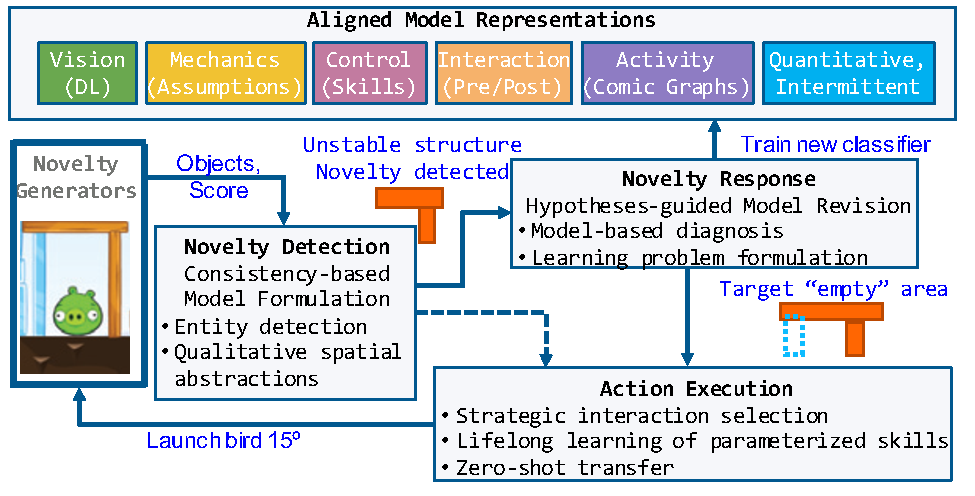
\includegraphics[scale=0.7]{figures/HYDRA.pdf}}
% \vspace{-0.3cm}
%         \caption{\label{fig:hydra} HYDRA draws on multiple model representations to plan actions, observe their effects, and focus learning.}
% \end{figure*}
% [[Roni: TODO Replace to a clearer figure that is more closely related to how we work]]
% Figure \ref{fig:hydra} shows an overview of Hydra. 
%Science Birds provides the score for the level and a description of the objects.


% HYDRA classifies these objects into types in its domain theory, and assesses if they have behaved consistently with the domain theory's expectations. These expectations could be driven by quantitative or qualitative composable models. Any inconsistencies are localized to model components using model-based diagnosis and learning problems are formulated. For example, if HYDRA does not understand why a structure has not fallen over, a possible explanation is that there is an unseen rigid object supporting it. Then, HYDRA may generate a plan to satisfy the learning goal by shooting a bird in that area and look for evidence of rigid object mechanics.


% Hydra, higher-level
%To address the novelty detection and response challenges in the persistent single novelty setup, we propose the \hydra agent and describe it here in detail.


\begin{figure}
	\centering
	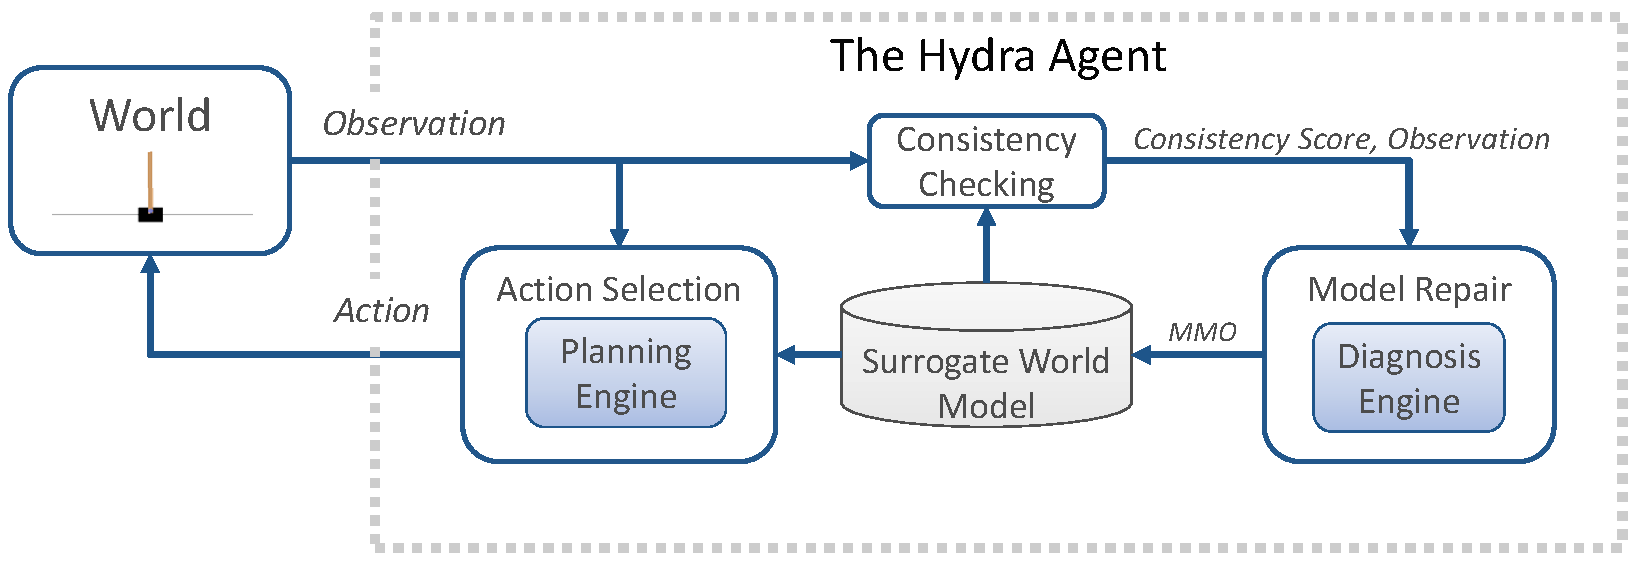
\includegraphics[width=\columnwidth]{hydra-cropped.pdf}
	\caption{An overview of an \hydra agent.}
	\label{fig:hydra-overview}
\end{figure}

% Surrogate model
\hydra assumes the availability of a compositional model $\hat{E}$ of the environment $E$ that can make predictions about the expected outcome of the agent's actions. 
Obtaining a compositional model for a given domain can be done manually by human experts  
or learned from data by action model learning algorithms such as ARMS~\cite{wu2007arms}, LOCM~\cite{cresswell2013acquiring}, FAMA~\cite{aineto19learning}, and SAM Learning~\cite{juba2021kr} and others~\cite{asai2020learning}. 
Recent work has even demonstrated learning such models from natural language~\cite{feng2018extracting,lindsay2017framer}. 
Note that while hydra has access to the compositional model $\hat{E}$, it may not have complete knowledge of the actual environment $E$, and, more importantly, to the environment after novelty has been introduced ($\varphi(E)$). 


% How it is used
\noindent \hydra has the following main modules. 
\begin{itemize}
\item \textbf{Action Selection.} The role of this module is to select which action to perform next given the current observed state in the environment.
\item \textbf{Consistency Checking.} The role of this module is to associate an \emph{inconsistency score} for the current observation, indicating how consistent it is with $\hat{E}$. A high inconsistency score indicates $\hat{E}$ and $E$ are not sufficiently aligned, possibly suggesting that novelty has been introduced. 
\item \textbf{Model Repair.} The role of this module is to modify the relevant components of $\hat{E}$ such that it is consistent with the recent observations. 
\end{itemize}

Figure~\ref{fig:hydra-overview} illustrates how these modules operate together. 
When the agent collects a new observation from the environment, it associates it with a consistency score using the Consistency Checking module. 
If the inconsistency score is reasonably low, \hydra finds a state $\hat{s}$ in $\hat{E}$ that best represents the current state in $E$ and selects the next action to perform using the Action Selection module. 
This is done by running an automated planner to generate a plan that starts at $\hat{s}$ and is expected to  maximize the collected reward according to $\hat{E}$.\footnote{Practically, one may wish to limit the number of planning sessions to save computational efforts.} 
Based on this plan, the Action Selection module outputs the next action to perform. 
This process continues until an episode is completed. 
At this stage, the Consistency Checking module analyzes the executed trajectory to see if it is consistent with $\hat{E}$. 
This means analyzing every observed transition, i.e., every $\tuple{\hat{s}, a, \hat{s}',r}$ tuple to see if all states and transitions are consistent with $\hat{E}$. 
If this is the case, no change to $\hat{E}$ is needed and \hydra will start a new episode. 
Otherwise, the Consistency Checking module outputs a real value $\gamma$ quantifying the likelihood that this consistency indeed indicates that novelty has been introduced. 
If this value passes some pre-defined threshold, \hydra declares that novelty has been detected. 
This inconsistency value is then passed to the Model Repair module along with the observed trajectory. 
%The MMR applies model-based diagnosis to suggest hypotheses explaining why the observed trajectory is inconsistent with $\hat{E}$. 
The Model Repair module attempts to modify $\hat{E}$ such that it will be consistent with the observed trajectory. 
This is done by applying a model-based diagnosis engine, e.g., GDE~\cite{dekleer1987diagnosing}, to identify the model components that explain the observed inconsistency. 
To this end, \hydra requires a set \emph{Model Manipulation Operators} (MMOs), denoted $\mathcal{M}$. 
Each MMO represents a possible change to $\hat{E}$. 
The Model Repair searches for a sequence of MMOs such that, when applied to $\hat{E}$, yields a model that is most consistent with the observed trajectory.  
Then, the selected MMO is applied to $\hat{E}$, and the process repeats for the next episode with the repaired meta model. 


\section{Implementing \hydra Agents using PDDL+}


\begin{figure}
	\begin{center}
		% \begingroup
		\fontsize{8pt}{10pt}\selectfont
		\begin{verbatim}
			(:process movement
			:parameters ()
			:precondition (and (ready)(not (total_failure)))
			:effect (and (increase (x) (* #t (x_dot)) )
			(increase (theta) (* #t (theta_dot)))
			(increase (x_dot) (* #t (x_ddot)) )
			(increase (theta_dot) (* #t (theta_ddot)) )
			(increase (elapsed_time) (* #t 1) ) ))
		\end{verbatim}
		% \endgroup
		\caption{(CartPole) Continuous PDDL+ process updating over time the positions and velocities of the cart and pole.}
		\label{fig:process-cartpole}
	\end{center}
\end{figure}


Next, we describe an implementation of a \hydra agent using PDDL+~\cite{fox2006modelling} as our modeling language for $\hat{E}$. 
PDDL+ is an extension of the well-known Planning Domain Definition Language (PDDL)~\cite{mcdermott1998pddl} that allows modeling of temporal hybrid systems as planning domains that exhibit mixed discrete and continuous system dynamics.
In PDDL+, actions are defined by specifying their preconditions and effects in PDDL. 
In addition, PDDL+ supports modeling exogenous behavior with discrete events and continuous processes.
Events apply discrete effects instantaneously, whereas processes apply changes over time while their preconditions hold. The agent has no direct control over processes and events, it can only interact with exogenous activity indirectly. 
Figure~\ref{fig:process-cartpole} demonstrate a process defined in PDDL+ for the movement of a cartpole. 
We chose PDDL+ since it generalizes many previously proposed planning languages, which highlights the generality of our approach and simplifies supporting additional domains. 
Also, there exists off-the-shelf PDDL+ planners, such as UPMurphi \cite{della2009upmurphi}, which can be used to obtain plans. 

 

%  \todo[inline,color=green]{[[Roni: Wiktor, can you put 2 small snippets of PDDL from the two domains here? nothing too large]]}
% When our agent receives a \sbirds level to play, it automatically translates it to a PDDL+ planning problem under our \sbirds PDDL+ model. Then, we use an off-the-shelf PDDL+ planner, UPMurphi \cite{della2009upmurphi}, to obtain a plan. 




\subsection{Consistency Checking}
%\subsection{Adapting to Novelty as Search in the Space of PDDL+ Model Manipulation Operators}
In simple terms, consistency is a measure of how accurately the compositional model of the environment describes the actual environment and its dynamics.
Given a PDDL+ model $\Pi$ and plan $\pi$, one can simulate the trajectory we \emph{expect} to observe when executing $\pi$. 
Our implementation of the Consistency Checking module computes the consistency score of an observed trajectory by measuring how different it is from the expected trajectory. 
In our implementation, we measured difference by computing the maximal Euclidean distance 
between matching states along these trajectories (i.e., tracking differences between the \textit{expected} and \textit{observed} positions and velocities of the cart and pole over the course of an episode). 
However, other ways to measure distances between trajectories can also be applied. 
A novelty is detected when the discrepancy between the observed and expected sequence of states exceeds a predefined threshold. 


This approach to detecting novelties is domain-independent. 
However, it relies on the accuracy of the PDDL+ model. 
In our implementation, this was sufficient for the Cartpole domain.
However, for other domains the available PDDL+ model may not be accurate enough to exactly match the observed state trajectory.
%Note that it was accurate enough to allow the off-the-shelf PDDL+ planner to create plans that yielded state-of-the-art results in the non-novelty version of \sbirds. 
To address this, one may augment the PDDL+-based Consistency Checking approach by creating a domain-specific consistency checking module that incorporates qualitative analysis of the observed and expected trajectories. Alternatively, one may employ representation learning and train a neural network over non-novelty episodes to do next state prediction. 
%(2) Created a domain-specific consistency checking component that incorporates qualitative analysis of the observed and expected trajectories. In particular, we matched the initial trajectory of the bird that was shot, the set of blocks destroyed at the end of each shot, and the types of objects that appears in the level. The current implementation of the \sbirds' consistency checker is a work-in-progress, and improving its accuracy is a topic for ongoing research.  \todo[inline,color=green]{[[Roni: not sure how to say all this in a nice way. Maybe push this to the experiments, Klenk: Agreed Just Replace the Sentence and say something like, \hydra combines these sources of information to perform novelty detection. Wiktor: I edited it to sound a bit more researchy, see what you think.]]}


% Roni: I can add a paragraph here with more details on how this consistency check was implemented currently. 

% % \subsection{Adapting to Novelty as Search in the Space of PDDL+ Models}
% Following Langley's recent \emph{Theory of Environmental Change}~\cite{langley2020open}, 
% we view novelty as a \emph{transformation} of the underlying world model. 
% To adapt to novelty, \hydra must update its domain model. To accomplish this, 
% it searches for a hypothesis 
% about the transformations that would be consistent with the observations. \hydra uses a set of \emph{Model Manipulation Operators} to transform the PDDL+ domain theory. To check if a sequence of MMOs is consistent with the observations, we apply them to the current PDDL+ model, 
% simulate the expected sequence of states according the modified model, 
% and check if this sequence of states is consistent with the sequence of states observed in the game. 
% After a consistent model has been found, it is used by HYDRA to generate future plans. 

\subsection{Meta Model Repair}


% \subsection{Adapting to Novelty as Search in the Space of PDDL+ Models}
The key to implementing a PDDL+-based \hydra agent is to define appropriate MMOs. 
For a PDDL+-based \hydra agent, an MMO is a function that modifies some element of the PDDL+ model, e.g., change an action, event, or process, or even add a completely new event or process. 
In our implementation, we limited the MMOs we consider to only modify the different constants used in the PDDL+ model, e.g., changing the constant corresponding to gravity by some fixed amount (either positive or negative). 


To check if a sequence of MMOs should be used, we apply a model-based diagnosis approach, that is, we apply them to the current PDDL+ model, simulate the expected sequence of states according the modified model, and check if this sequence of states is consistent with the observed trajectory using the Consistency Checking module. 
The space of possible MMO sequences is combinatorial. 
To focus the search, a model-based diagnosis engine can be used. 
We implemented 
To search this space, we implemented a greedy best-first search that uses a heuristic a linear combination of the consistency score returned by the consistency checker and the size of the evaluated MMO sequence. 
The latter consideration biases the search towards simpler repairs. 


%This implementation of the MMR is domain independent and is, in fact, the exact same source code for both domains. However, in general, the set of possible MMOs to use for the meta-model repair is a domain-specific design choice. We discuss these choices later in the Discussion section. 

%There may be multiple models consistent with the current observations. Also, new novelties may occur over time. Therefore, the process of detecting novelties and adapting HYDRA's PDDL+ model to them is continuous: after every action HYDRA performs, it checks if the current observation is consistent with its model. If it is not, it searches for a sequence of MMOs that would yield a model that is consistent with the current and previously collected observations. 






\section{Experimental Results}

% [[Roni: maybe add some text about the optimal closed-loop control formulae? or the one we used? not sure about this]]
% @article{yu2008closed,
	%   title={Closed-loop tracking control of a pendulum-driven cart-pole underactuated system},
	%   author={Yu, Hongnian and Liu, Yang and Yang, Taicheng},
	%   journal={Proceedings of the Institution of Mechanical Engineers, Part I: Journal of Systems and Control Engineering},
	%   volume={222},
	%   number={2},
	%   pages={109--125},
	%   year={2008},
	%   publisher={SAGE Publications Sage UK: London, England}
	% }
% @inproceedings{duan2016benchmarking,
	%   title={Benchmarking deep reinforcement learning for continuous control},
	%   author={Duan, Yan and Chen, Xi and Houthooft, Rein and Schulman, John and Abbeel, Pieter},
	%   booktitle={International conference on machine learning},
	%   pages={1329--1338},
	%   year={2016},
	%   organization={PMLR}
	% }

\todo{Editted the next paragraph, please review}
Next, we demonstrate the ability of our PDDL+-based \hydra agent to detect and respond to novelty effectively by performing experiments on the well-known balancing Cartpole domain. We also report on a small-scale comparison with an off-the-shelf RL agent, showing that \hydra can respond effectively to some novelties using significantly fewer interactions with the environment. 
%In this section, we report on a small-scale demonstration of our PDDL+-based \hydra agent on the well-known balancing Cartpole domain. 

\subsection{The Cartpole Domain and Novelties}

\todo{Edited the next paragraph, please review}
The Cartpole domain is a classical RL benchmark in which a pole is connected to a cart and the task is to balance the pole in the upright position by pushing the cart either left or right. 
There are multiple variants to the Cartpole domain. 
In our experiment, we used the standard Cartpole implementation 
from OpenAI Gym (https://gym.openai.com). 
This Cartpole domain is defined by several parameters including mass of the cart, length of the pole, gravity, and friction coefficient. 
A state in this domain is represented by 4 state variables (velocities and positions of the cart and the pole).
In every step, the agent's action is to apply force to the cart in either left or right direction. 
An episode ends when either 200 steps have been performed or a limit is exceeded (i.e. pole angle or cart position). % [[TODO: min/max angle]]. 
Every step returns +1 reward, so the total reward for an episode is between 1 and 200. 


We ran experiments where the introduced novelty involves changes the values of the pole's gravity and the mass of the cart. We experimented with a range of changes to these values. The results reported are for two such changes: 
(1) \emph{Type 1}: gravity increases from $9.8$ to $12$ and the pole length grows from $1.0$ to $1.1$;
(2) \emph{Type 2}: cart mass decreases from $1.0$ to $0.9$ and the pole length grows from $1.0$ to $1.1$. 
We selected to report on these types of novelties as introducing them resulted in a significantly decrease in performance for all agents but the cartpole in the environment after introducing is still controllable.  
The selected novelty type was introduced in the $8^{th}$ episode in a trial. 
Every trial consisted of $30$ episodes, and each experiment consisted of $5$ trials.

%\todo[inline,color=green]{Wiktor: why these novelty values? If we have space, perhaps we should mention that these values were selected to keep the game playable, but have significant effects on performance, or something along those lines.} Roni: good call. Added above text for this. 


%We are interested in designing adaptive systems that can deal with novelties introduced during their deployment robustly. There are two desired properties of such systems. First, they should detect and react to novelty \emph{quickly} with few interactions with the environment. This is desired because often, it is infeasible to collect large amounts of data during deployment. Secondly, the adaptation in the system should be \emph{interpretable} by a human. This dimension is useful for adaptation during deployment as it enables a human designer or operator to inspect why the system behavior has evolved and ascertain if that adaptation is correct. Below we evaluate our proposed approach in \hydra along these dimensions and analyze its performance. 

% \todo[inline,color=green]{TODO: Shorten paragraph above}

%\textbf{Experiments} Our experiments were conducted in the CartPole domain. 
% \todo[inline,color=green]{Ideally, we would put here the analytical control solution for this, which uses all these parameters and explain them. Not critical}

\subsection{Baselines and Experiment Setup}

In addition to \hydra, we report on the performance of two baseline agents: a non-adaptive planning agent and a deep Q-network (DQN) reinforcement learning agent. 
We refer to these agents as the planning agent and DQN agent, respectively. 
The planning agent uses the same PDDL+ modeling and planner as \hydra, but does not attempt any model repair.  
The DQN agent uses a standard deep q-network implementation with experience replay memory \cite{mnih2013playing}. It is built with an input layer ($4 \times 16$), a hidden layer ($16 \times 16$), and an output layer ($16 \times 2$) and uses the Rectified Linear Unit (ReLU) activation function.   
Both baseline agents were designed and trained to achieve perfect performance in the non-novelty case prior to the experiment. 



The experiments we performed involved running each agent through a series of trials. 
Each trial starts by running the agent through a sequence of episodes in the non-novel environment. 
Then, we introduce one of the novelty types described above to the environment, and continue to run the agent on episodes from the now novel environment. 
The performance of the agent on the non-novel episodes reflects its performance on the environment it has been designed or trained for, while the performance on the novel episodes measure its ability to respond to the introduced novelty. 


\todo{Edited this. Good if someone reads it again.}
We conducted two types of experiments: (1) \emph{system detection} experiments, in which the presence of novelty was not indicated to the agent and it is expected to infer the presence of novelty and react to it autonomously, and (2) \emph{given detection} experiments, in which an oracle indicated the presence of novelty to the agent. 
Given detection experiments allow us to measure separately the agent's ability to respond to novelties, while system detection experiments better simulate how agents act in the real-world, where novelty detection oracles are not available. 
The planning agent does not attempt to learn or adapt to novelty, so its behavior for both experiment types (system detection and given detection) is the same. 
The DQN agent does not explicitly attempt to detect novelty, thus its behavior in the system detection experiments is to continue to run with its trained Q-network. 
For the given detection experiments, we allow the DQN agent to reset its learning factor and make Bellman updates to its trained Q-network when novelty is indicated.  


%The system detection experiment simulates the real-world, while the second type of experiment to allow measureing separately the agent's ability to detect novelty and respond to it. 


% \textbf{Baselines} In addition to \hydra, we report performance to two baseline agents: 
% a non-adaptive planning agent and a deep Q-network (DQN) reinforcement learning agent. 
% We refer to these agents as the planning agent and DQN agent, respectively. 
% These baseline agents were designed and trained to achieve perfect performance in the non-novelty case prior to the experiment. 
% The planning agent does not attempt to learn or adapt to novelty, and so its behavior for both experiment conditions (system detection and given detection) is the same. 
% The DQN agent makes Bellman updates to its trained Q-network when novelty was indicated to it in the given detection experiment condition.  
%  \todo[inline,color=green]{What about the learning factor? do we reset it to learn from scratch?}

\subsection{Results}

\begin{figure*}
    \centering
    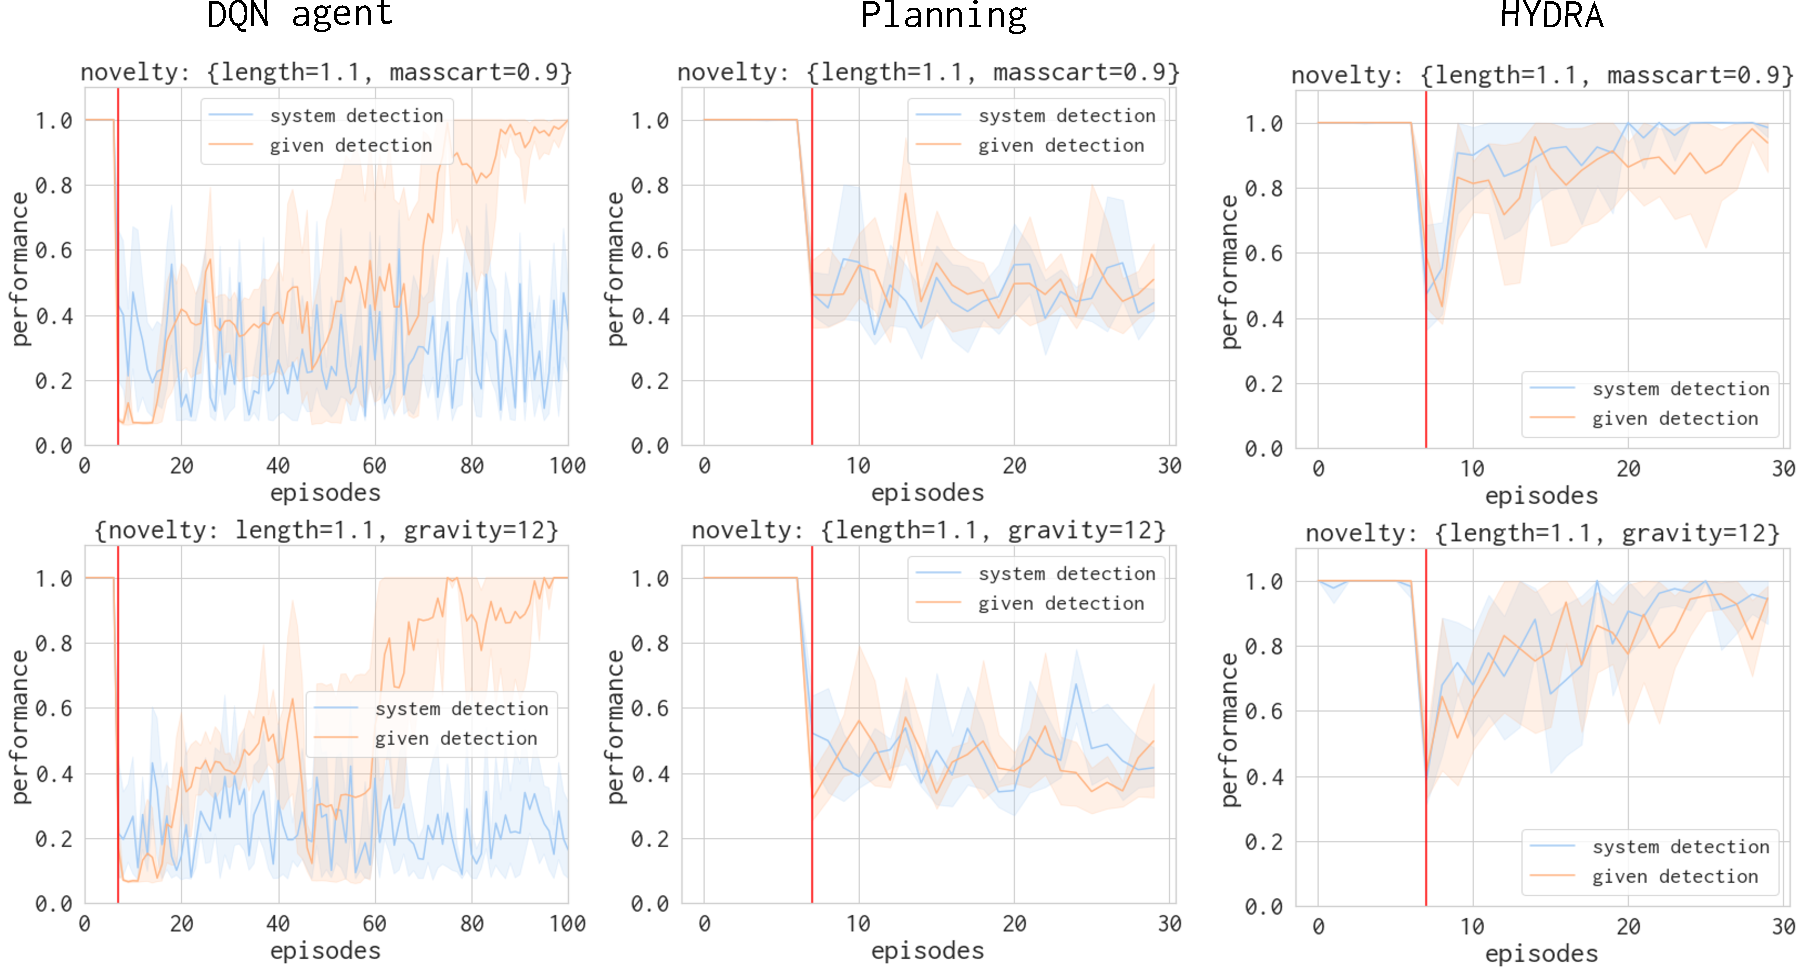
\includegraphics[width=0.85\textwidth]{figures/experiments/compiled-results.pdf}
    %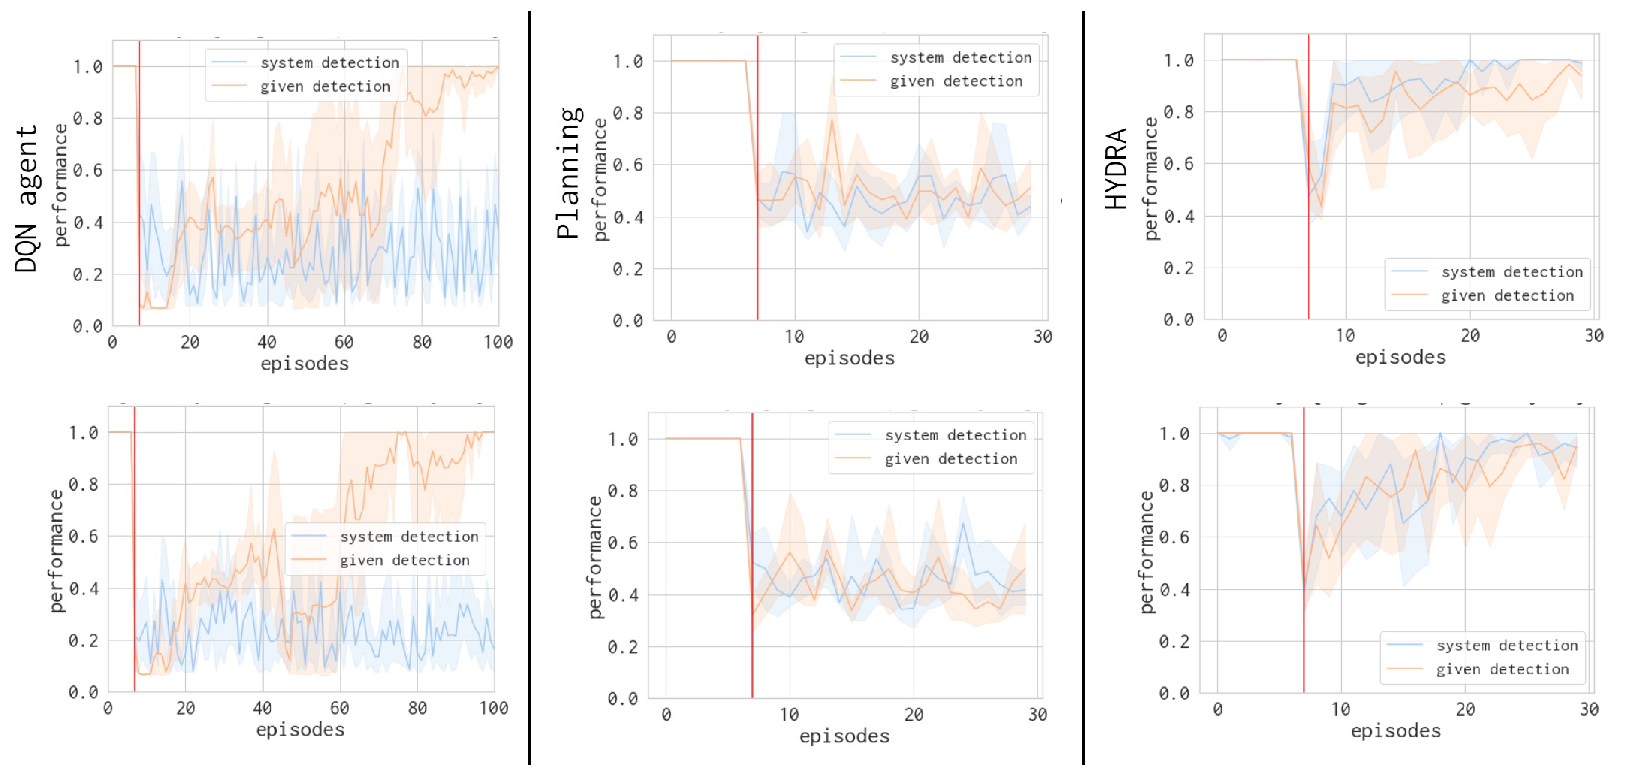
\includegraphics[width=0.85\textwidth]{figures/experiments/hydra-results.pdf} 

    \caption{Graphs showing performance of DQN agent, planning agent, and \textsc{hydra} in novelty experiments. Episodes in a trial are on the x-axis and reward earned is shown on the y-axis. The results are averaged over $5$ trials. Red line indicates the episode where novelty has been introduced. In the top row, the novelty introduced is increasing the pole length to 1.1 and decreasing the cart mass to 0.9 (novelty type 1). In the bottom row, the novelty introduced is the same increase in pole length and setting gravity to be 12. The results clearly show that \hydra adapts very quickly to the novelties in our experiment, returning to optimal performance in ~10 episodes.}
    \label{fig:combined-results}
\end{figure*}


The results are summarized in Figure \ref{fig:combined-results}. The $x$-axis shows the episodes in a trial and the $y$-axis shows the total reward collected by the agent per episode, represented as the proportion of its score with a perfect controller. 
The red line indicates the episode where the selected novelty was introduced. 
The blue line shows the results for the ``system detection'' experiments and the orange line shows the results for the ``given detection'' experiments. The shaded areas for each represent the $95\%$ confidence interval computed over $5$ trials.
\todo{@Shiwali: what are the shaded colors around the line? std. dev.? also, how many experiments were run?}


% Trend 1: Composable models are more robust
As shown in Figure \ref{fig:combined-results}, all agents achieve perfect performance at the beginning of the trial and then experience a significant drop in performance as soon as the novelty is introduced (episode $8$). This shows the selected novelties are meaningful for all agents. The are three key observations to be made.
  %The behavior changes in characteristic ways after the novelty is introduced.
%Then, all agents experience a drop in performance as soon as the novelty is introduced in episode $8$. 
%is expected because the agents' were designed to operate in the non-novelty settings. 
%Their models (and Q-functions) become outdated and lead to worse performance. 

\emph{Resilience}: The performance drop observed when novelty is introduced is significantly more drastic for the DQN agent than for the planning agent and \hydra. For both types of novelties, the performance of the DQN agent drops to approximately $25\%$ of its pre-novelty performance and below, while the performance of the planning agent and \hydra drop by only $50\%$. 
This difference can be explained by the agents' design. 
Both the planning agent and \hydra are built with \emph{composable} component models. 
Even in novel situations, a majority of the component models are still relevant and can be exploited to drive behavior. 
In contrast, the knowledge that drives behavior in end-to-end learning systems like the deep Q-network is distributed and cannot be re-purposed to drive behavior in an environment with changing dynamics. 
This observation demonstrates that agents based on a composable component models can be reselient to novelties.

% Trend 2: Only hydra adapts 
\emph{Quick adaptation}: Since the planning agent does not react to novelties directly, its performance does not improve over time in both experimental conditions (given detection and system detection). 
The DQN agent does attempt to adapt to the observed novelty. While it starts with worse performance in the given detection condition, it improves towards the later parts of the trial. 
This observation suggests that the agent is learning a new Q-function that supports the new dynamics of the environment under novelty conditions. 
However, this learning is slow, requiring multiple interactions with the environment to return to optimal performance ($\sim75$ episodes). 
In contrast, \hydra adapts very quickly in less than $20$ episodes for all the types of novelty and experimental conditions we considered. 
This observation supports our central thesis: \hydra's model-based design enable fast novelty response via localized novelty detection and adaptation. 
\todo[inline,color=green]{IMPORTANT: How did the DQN detect novelty in the system detection case? did it use the PDDL+ consistency checker? or some other method? Maybe best to remove the blue line from the DQN and planning agents. [Wiktor: 1. I assumed that the DQN agent would try to learn from playing and improve its performance over time, but that it holds no information about novelty existence, is that the case? if so, then why the discrepancy between the blue and orange lines?
2. the DQN agent learns while playing, right? then why does the blue line not climb?][Roni: Shiwali explained to me: blue line means it does not continue to learn, orange line means it starts to learn from scratch when novelty is introduced. I'll fix the text accordingly}

%, making the corresponding learning very efficient. 
% \hydra performs similarly in both experimental conditions, suggesting that \hydra can reliably detect novelty even when it is not indicated using consistency checking. 
%   \todo[inline,color=green]{Ideally, we would hav novelty detection results for these novelties to support this} Roni: I am concerned about this conclusion and feel it is not supported by our results. 


% \begin{figure}
%     \centering
%     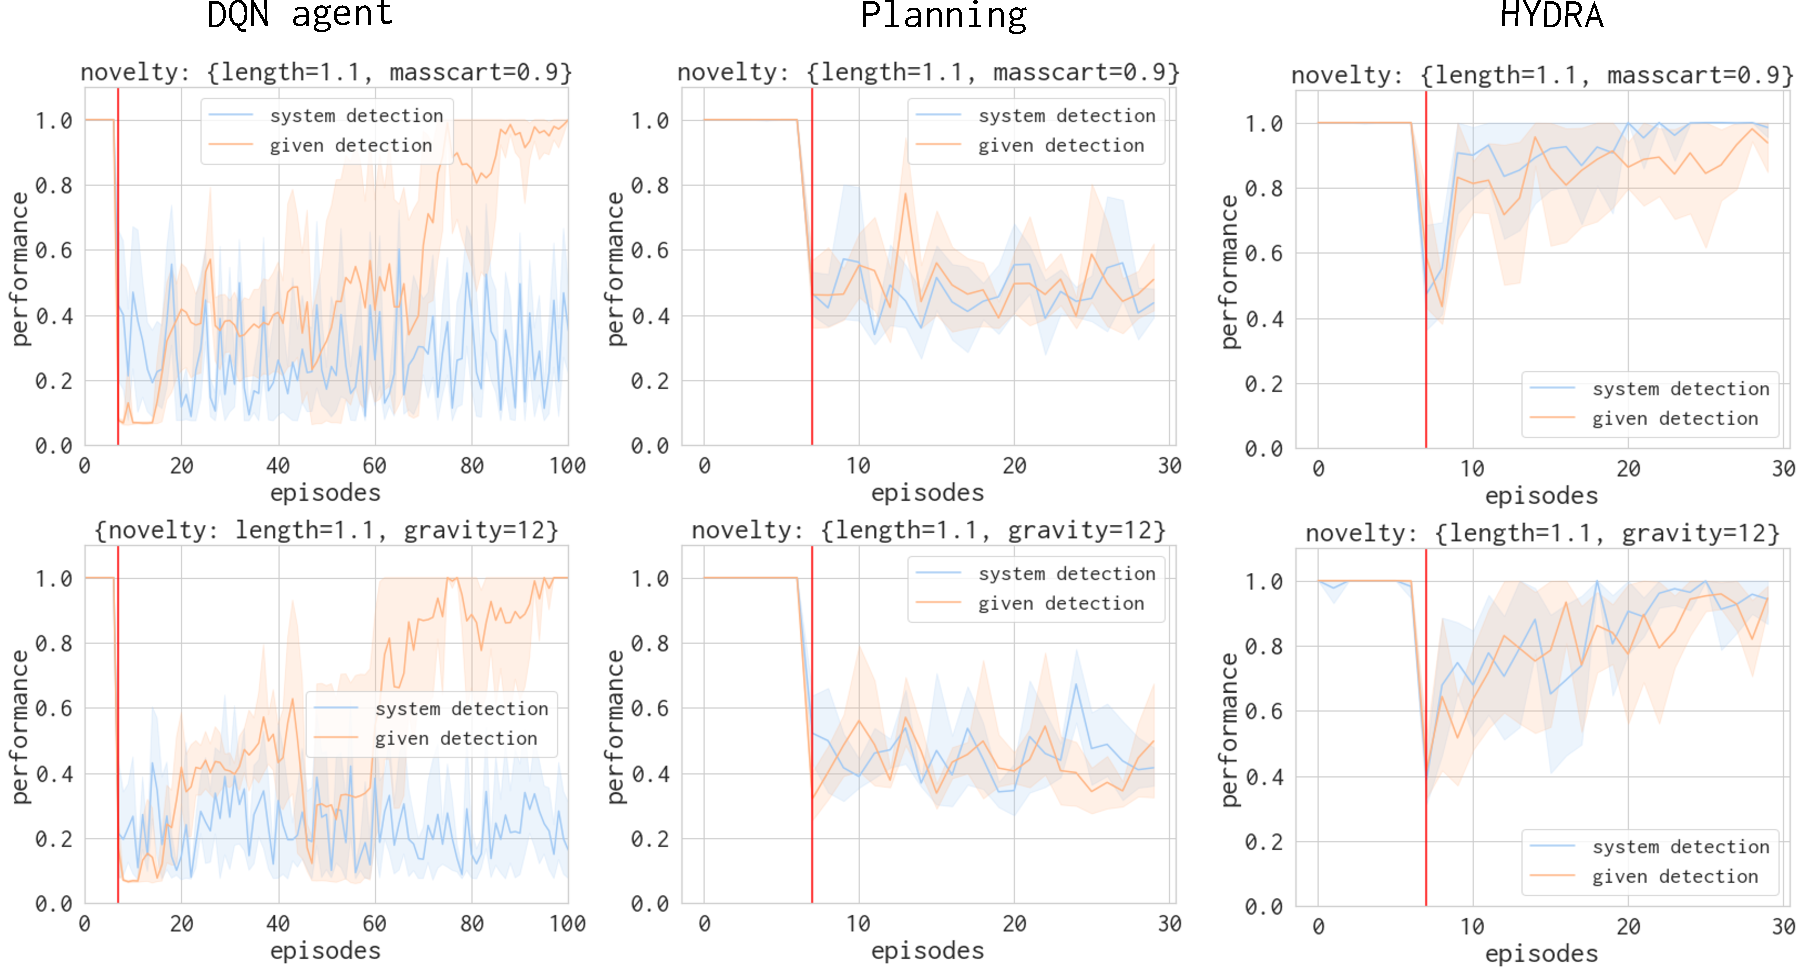
\includegraphics[width=0.5\textwidth]{figures/experiments/compiled-results.pdf} 
%     \caption{Total reward (y-axis) for each episode (x-axis) in a trial. Red line indicates the episode where novelty has been introduced. 
%     	The results clearly show that \hydra adapts very quickly to the novelties in our experiment, returning to optimal performance in ~10 episodes.}
%     \label{fig:combined-results}
% \end{figure}



\emph{Interpretability}: \textsc{hydra} adapts to presented novelties by proposing how various elements of its model of the environment can be changed and consequently, its learning can be inspected an analyzed by a human. Figure \ref{fig:example} shows examples of adaptation in hydra in response to the posed novelty of Type 2. 

\begin{figure}
    \centering
    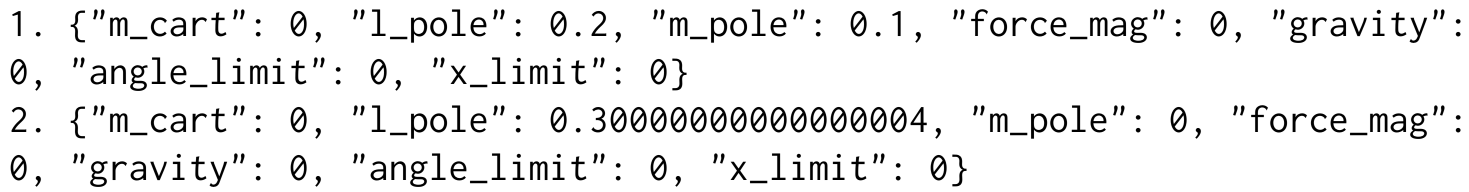
\includegraphics[width=0.5\textwidth]{figures/experiments/inspectable.png}
    \caption{Example adaptations produced by \textsc{hydra} represented as changes to various elements in the model (presented as delta from the default value of each variable, 0 denotes no change).}
    \label{fig:example}
\end{figure}

\todo{Modified and moved this to here. Comments and edits are very welcome.}
   %\todo[inline,color=green]{Last sentence is tricky? [roni: I think it is Ok]}

% \subsection{Cartpole}

% \subsubsection{Novelty Detection}
% Ideal trend: a human-generated composable model is more effective in detecting novelty than black box approaches. 

% Task 1: Compare Hydra novelty detection against an off-the-shelf anomaly detection algorithm. 

% Concrete task:
% Compare the UPenn model with our Cartepole novelty detection over the benchmark
% Metrics: FP, FN, ...

% Shiwaliwill help here

% Question: can the UPenn model be considered an off-the-shelf anomaly detection?
% \begin{figure}
%     \centering
%     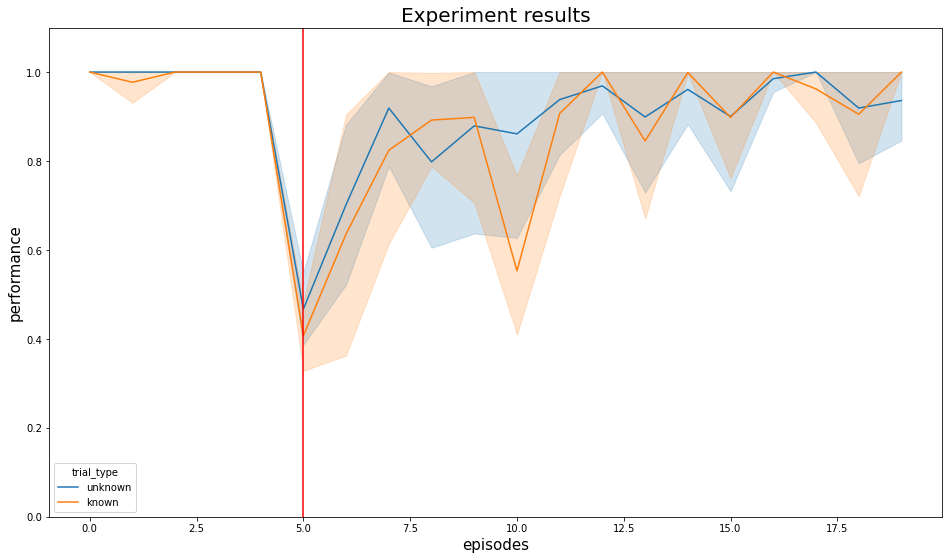
\includegraphics[width=0.5\textwidth]{figures/repairing-cartpole.png}
%     \caption{Caption}
%     \label{fig:my_label}
% \end{figure}



% \subsubsection{Novelty Response}
% Ideal trend: a human-generated composable model with our diagnosis-based approach allows faster adaptation to novelty 

% Task 2: Compare Hydra performance after novelty with an off the shelf RL approach 
% and also a non-adaptive Hydra agent (e.g., just a planner)


% \subsection{ScienceBirds}
% \subsubsection{Novelty Detection}
% Task 3: the same but more refined: here the model is not perfect, but we need both system 


% To compare the different novelty detection methods --- NN-based, PDDL-based, and the NN-PDDL hybrid (denoted Hybrid hereonafter) --- we performed the following set of experiments. 
% In each experiment, we run our agent with each of the novelty detection methods (NN, PDDL, or Hybrid) on a trial with 20 levels. 
% Novelty is being introduced after the first 10 levels are played. 
% We repeated this experiments with each of the 13 novelties published by ANU in the ScienceBirds novelty competition track.\footnote{\url{aibirds.org/angry-birds-ai-competition/novelty-track.html}} 
% After every level, the agent reports whether it detected novelty or not, and we evaluted the novelty detection method by measuring the number of false positives (novelty detection reported by the agent although no novelty has been introduced) and false negatives (novelty introduced by not detected by the agent). 

% \begin{figure}
%     \centering
%     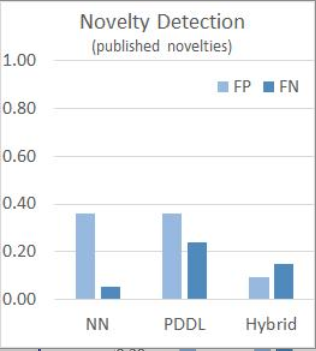
\includegraphics[width=0.7\columnwidth]{figures/SB-Novelty Detection.png}
%     \caption{Average false positives and false negatives rates in the ScienceBirds domain using different novelty detection methods.}
%     \label{fig:sb-detection-experiment}
% \end{figure}

% Figure~\ref{fig:sb-detection-experimentmy_label} shows the results of these experiments. The results show that the NN-based and PDDL-based detection alone yield a high false positive rate of over 0.3, while the NN-PDDL Hybrid detection has a false positive rate of approximately 0.1. 
% This comes at some cost to the amount of false negatives, which is slightly smaller for the NN-based detection. 


% \subsubsection{Novelty Response}
% Task 4: the same

% We don't have a standard RL approach

% Question: is there an off the shelf RL approach for SB
% Wiktor will look for this?




\section{Related Work}

The topic of how to detect and react to novelties has been gaining significant attention in the AI literature. 
The novelty problems we address in this work has been described by Senator~\cite{senator2019sailon} 
and analyzed by Boult et al.~\cite{boult2021towards}
and Langely~\cite{langley2020open}. 
Boult et al.~\cite{boult2021towards,langley2020open} did not propose an agent design for this setting, but rather suggested a framework for characterizing different types of novelties. 


Langely also identified four elements an agent architecture needs to properly address novelty detection and response --- ``performance, monitoring, diagnosis, and repair.'' 
\hydra implements these elements. 
It uses its meta model to generate plans, act (\emph{performance}), and detect novelties (\emph{monitor}). 
Then, it uses heuristic search to identify elements of the meta model that are incorrect (\emph{diagnosis}) and modifies the meta model accordingly (\emph{repair}). 

We are not the first to design a novelty-robust agent and novelty detection and response algorithms. DiscoverHistory~\cite{molineaux2012discoverhistory} is an algorithm for inferring the possible values of unobservable state variables from observations. While our current experiments are similar in nature, HYDRA is designed to be more general, including novelties such as adding new variables, process, and object types. MIDCA~\cite{paisner2014goal} is a cognitive architecture for designing novelty-robust agents, where novelty is limited to which goal to pursue next. The recently proposed OpenMIND system~\cite{musliner2021openmind} addresses as similar problem setup to ours, but on a different set of domains and using a less expressive planning formalism. \todo{Last line is newly added. Please read. Not strong enough IMO.}


% \todo[inline,color=green]{[[TODO: Mention Pat Langley's paper, Mention Terry's Boult's paper, also SIFTS work if they have one yet, Roni: I didn't see any recent paper by David M so I'm assuming they don't have anything yet]]}

%More recently, there have been attempts at defining more general frameworks for handling novelty in open-world environments, driven by our contemporaries from the DARPA-SAILON program.[[Roni: No no, we're an anonymous author]]
More recently, there have been attempts at defining more general frameworks for handling novelty in open-world environments. 
Muhammad et al. \shortcite{muhammad2021novelty} proposed an approach for a cognitive agent to detect, characterize, and accommodate novelties based on knowledge and inference from the agent's internal predictions and the observed ground truth. 
% As expected from a fellow research program participant, there are similarities in our approaches. 
While it also exploits a planning-centric architecture and defines the composition of the world in a planning paradigm, there exist differences, the key of which is the richness of the environments that our approaches operate in and reason with. Most notably, they do not consider scenarios with external activity (i.e. beyond the executive of the agent), or continuous change in the environment. 

Other recent developments in the area have tackled yet another class of application domains, such as the game of Monopoly \cite{gopalakrishnan2021integrating}, a multi-player game heavily skewed towards uncertainty (from dice rolls, card draws, or adversaries' actions). The agent behaves according to a policy with a state-value function based on a short-horizon lookahead approach, prioritizing robustness to novelties in an already unpredictable game. 


%Adapting to novelties can also be viewed as a special case of \emph{Life Long Learning}~\cite{thrun1998lifelong,eaton}. 

%thrun1998lifelong

\section{Discussion}



\begin{table}[tbh!]
	\centering
	\footnotesize
	\begin{tabular}{p{0.25\columnwidth} | p{0.35\columnwidth} | p{0.3\columnwidth}}
		\hline
		\textbf{Novelty types} & \textbf{Domain adjustment} & \textbf{Novelty examples} \\
		\hline
		Spatio-temporal  & Fluent changes & Increased gravity \\
		Structures  & New objects and fluents & Ball added to cart \\
		Processes  & New and/or changing existing processes & Introduced wind \\
		Constraints & New preconditions and/or changed events & Limit direction change frequency \\
		
		%Spatio-temporal Transformation & Fluent changes & Increased the force of gravity \\
		%Structures Transformation & New objects and fluents & Introduced new type of bird \\
		%Processes Transformation & New and/or changing existing processes & Introduced wind \\
		%Constraints Transformation & New preconditions and/or changed events & Only explosions can kill pigs \\
		\hline
	\end{tabular}
	\caption{Description of example novelties that can be encountered in cartpole, changes to the PDDL+ model required to accommodate them, and their corresponding novelty types  defined by~\protect\cite{langley2020open}.} % TODO RONI!!!!! \cite{langley2020open}.}
\label{tab:novelties_pddl}
\end{table}

Most modules in the \hydra agent are domain-independent and we are currently implementing it on two other domains that can be expressed using PDDL+. 
To implement \hydra in a new domain that can be represented by PDDL+, one needs to only (1) create the initial PDDL+ compositional model, and (2) select the appropriate MMOs for the Model Repair module.
%There are two domain-specific parts A challenge in the design of \hydra is how to select the appropriate set of MMOs. 
In our current implementation, we focused in MMOs that modify the value of constants in the PDDL+ model such as gravity, pole length, and pole mass. 
% the force gravity applies on flying objects, the size of the birds, and the speed in which the slingshot's angle is adjusted.  
An open research challenge is how to identify the necessary and sufficient set of MMOs for a given domain and types of novelties. 
Table~\ref{tab:novelties_pddl} maps possible types of MMOs to types of novelties as defined by Langley~\cite{langley2020open} along with examples from the cartpole domain. 
%from \sbirds, one of the domains we are implementing \hydra for.
% [[Roni: I decided not to detail more here, mainly due to time. Let me know if you think more is needed]
% [[Roni: I copied some of the text about this to drafts.tex]
The number of MMOs may be very large and thus finding a sequence of MMOs that may yield a consistent model is a challenging combinatorial search problem.  We expect to need heuristics to guide the search in an efficient manner. 
In our current implementation, we run a Greedy Best-First Search algorithm that uses a heuristic that prefers shorter MMO sequences that yield models that are more consistent. Future work may explore more sophisticated search techniques for this task. % Roni: this is pretty vague, but it is what I did. If this was not an abstract and we had more time , I'd say more. Let me know what you think



The requirement to define MMOs a-priori also raises the question: how will \hydra work on novelties that cannot be property characterized with the selected set of MMOs. Indeed, \hydra will fail if no sequence of MMOs can reach a compositional model that sufficiently captures the novel aspects of the environment. However, note that even if the MMOs do not allow exactly defining the modifications to the environment, they might still allow finding a compositional environment model that is close enough to allow reasonable action selection. 
\todo{New paragraph below, please read}
For example, consider the case where the novelty introduced is an increase in air resistance, but the available \hydra agent only has an MMO that modify the amount of force applied to the cart when pushed by the agent. The Model Repair module of \hydra might then apply that MMO and incorrectly repair its model to assume the force it applies is weaker than it really. While the new compositional model is different from the actual changed environment, it would allow effective acting for slow cart speeds. Nevertheless, such an agent will under-perform when the cart reaches higher velocities. 
More broadly, one may ask whether the novelty response problem is not amenable to a theory equivalent to the ``no free lunch'' theorem, where any novelty response solution will work on some novelties but fail on others. This is another topic for future work. 


\section{Conclusions and Future Work}
\todo[inline,color=green]


We presented an architecture for a model-based agent called \hydra, which can plan and act in an environment, as well as detect and adapt to novel changes in the environment as they occur. 
The key idea in the \hydra architecture is the use of compositional model of the environment. 
\hydra uses this model to (1) generate plans, using an automated planner; (2) detect novelties, by matching observations with model predictions; and (3) adapt to novelties, by applying model-basd diagnosis to identify the model components that need to be repaired. 
%to to plan which actions to perform, monitor their execution, detect changes in the environment and adapt to them. 
. %Mapping observations and actions from the environment to the surrogate environment model is done using a \emph{meta model} that describes such conversions. 
%To detect when novelty occurs, \hydra compares the observations it collects with the one it expects according to its surrogate environment model.
% To adapt to novelties, \hydra automatically attempts to repair its meta model based on observations. 
% This is done by diagnosing its surrogate environment model and observed trajectories, and employing model-based diagnosis to identify sequences of model manipulation operators (MMOs) that can make the surrogate model consistent with the observations.  
We described a complete implementation of \hydra using the PDDL+ to describe its compositional model of the environment.   
Finally, we empirically evaluated our PDDL+-based \hydra agent in the Cartpole domain, a well-known DQN benchmark.
Our results demonstrate several types of novelty that our PDDL+-based agent can detect and adapt to very rapidly, requiring at most 20 episodes before returning to normal performance, which is significantly faster than an off-the-shelf DQN for this domain. 



\bibliography{library}

% \section{Acknowledgments}
% AAAI is especially grateful to Peter Patel Schneider for his work in implementing the original aaai.sty file, liberally using the ideas of other style hackers, including Barbara Beeton. We also acknowledge with thanks the work of George Ferguson for his guide to using the style and BibTeX files --- which has been incorporated into this document --- and Hans Guesgen, who provided several timely modifications, as well as the many others who have, from time to time, sent in suggestions on improvements to the AAAI style. We are especially grateful to Francisco Cruz, Marc Pujol-Gonzalez, and Mico Loretan for the improvements to the Bib\TeX{} and \LaTeX{} files made in 2020.


\end{document}
